% Preprint — Hole suppression and absorption. Author: Derek Blair <derekjblair@gmail.com>
% Source data:
%   ~/workspace/math-unsolved/ROUND199_DOSSIER.md (2026-10-09): suppression
%     theory T1--T5, surveys (30 hole-capable pairs; 24 realized, 6 suppressed).
%   ~/workspace/math-unsolved/ROUND200_DOSSIER.md (2026-10-09): absorbed 13|h
%     regime, T2--T5', 30-quad census [COMPUTED].
%   ~/workspace/math-unsolved/ROUND230_DOSSIER.md (2026-10-09): Lean lane —
%     HoleSuppression.lean + AbsorbedRegime.lean moved [PROVED*]->[PROVED];
%     bakkie `lake build` exit 0, zero sorrys, axioms probes.
%   ~/workspace/math-unsolved/ROUND234_DOSSIER.md (2026-10-09): local
%     elaboration exit 0 (8925 jobs); R227 review outcomes.
%   ~/workspace/math-unsolved/ROUND238_DOSSIER.md (2026-10-09): hostile review
%     of R200 T2/T3/T4 — T2 FAILS as stated (13^1||R assertion), T4 FAILS as
%     stated (counterexample (321,13,1,16678)), corrected T4 review-validated;
%     AbsorbedBound.lean drafted. T3 review gate PASSED.
%   ~/workspace/math-unsolved/ROUND250_DOSSIER.md (2026-10-10): AbsorbedBound.lean
%     repaired, built exit 0 on bakkie and locally, zero sorrys,
%     standard-only axioms, md5-identical both sides; corrected T4 [PROVED].
% Lean modules (derekblair/math-proofs repo):
%   Mathproofs/HoleSuppression.lean — t2_iff, dichotomy_two_margins,
%     t5_saturation, t5_double_saturation, t5_sigma_one (+ uniqueness lemmas).
%   Mathproofs/AbsorbedRegime.lean — t5prime_combined, t5prime_R1/R2/R3/R6,
%     m_ge_three.
%   Mathproofs/AbsorbedBound.lean — t4_self_bound (+ 8 lemmas).
% All figures native TikZ/pgfplots; all tables booktabs; no external assets.
\documentclass[11pt,a4paper]{article}
\usepackage{amsmath,amssymb,amsthm}
\usepackage{stmaryrd}
\usepackage{tikz}
\usetikzlibrary{positioning}
\usepackage{pgfplots}
\pgfplotsset{compat=1.18}
\usepackage{booktabs}
\usepackage{geometry}
\geometry{margin=2.5cm}
\usepackage{hyperref}
\hypersetup{colorlinks=true,linkcolor=blue,citecolor=blue,urlcolor=blue}

\newtheorem{theorem}{Theorem}
\newtheorem{proposition}{Proposition}
\theoremstyle{definition}
\newtheorem{assumption}{Assumption}

\title{Hole Suppression and Absorption in Saturated Sidon Families}
\author{Derek Blair \\ \texttt{derekjblair@gmail.com}}
\date{October 2026}

\begin{document}
\maketitle

%======================================================================
\section{Abstract}
%======================================================================

This preprint formalizes two program-internal developments as
machine-checked Lean~4 theorems: the \emph{hole-suppression} theory of
Round~199 (the suppression coefficient~$\sigma(r)$ and the conditions
forcing it to~$1$) and the \emph{absorbed $13\mid h$ regime} of
Round~200 (the self-bounding $c\le 320$ arithmetic and the
$R\in\{1,2,3,6\}$ impossibility). Concretely:

\begin{itemize}
\item \textbf{HoleSuppression.lean}: the T2 dichotomy ---
  hole-capability is equivalent to having at least two non-singleton
  margins (\url{t2_iff}, with the constructive two-diagonal witness
  \url{dichotomy_two_margins}) --- and the T5 saturation-forcing
  lemmas (\url{t5_saturation}, \url{t5_double_saturation},
  \url{t5_sigma_one}): a bijective map sends \url{univ} to
  \url{univ}, so a saturated fiber cannot host a hole.
\item \textbf{AbsorbedRegime.lean}: the T5$'$ arithmetic kernel
  (\url{t5prime_combined} plus case lemmas
  \texttt{t5prime\_R1/R2/R3/R6}): with $m=4c-1$ and the per-$R$
  automaticity conditions, no quad with $R\in\{1,2,3,6\}$ is possible,
  in any regime.
\item \textbf{AbsorbedBound.lean}: the \emph{corrected} T4 self-bound
  (\url{t4_self_bound} plus eight lemmas): an absorbed quad with
  $R\mid30030$ satisfies $c\le320$.
\end{itemize}

All are \textbf{[PROVED]}: built on \url{bakkie} and locally with
\texttt{lake build} exit~0, zero \url{sorry}s, standard-only axioms
($\texttt{propext}$, $\texttt{Classical.choice}$, $\texttt{Quot.sound}$),
Lean~4.34.1 + Mathlib pinned at commit~\url{d13f23b}.

A central honesty element of this paper is the \textbf{refutation and
correction of the original T4}: the as-stated claim ``absorbed implies
$c\le320$'' is \emph{false} --- hostile review produced the explicit
absorbed counterexample $(c,h,a,b)=(321,13,1,16678)$, and in fact the
family $(c,13,1,52c-14)$ is absorbed for \emph{every}~$c$. The
machine-checked theorem above is the corrected statement, with the
$R\mid30030$ (non-dead) hypothesis restored. The R200 T2 trichotomy
extension was likewise demoted to [OPEN] (a false $13^1\Vert R$
assertion); T3's fiber-extruded slice survives review
([PROVED*], formalization pending). Table~\ref{tab:inventory} gives the
full claim inventory with statuses.

%======================================================================
\section{Introduction}
%======================================================================

This paper publishes the Lean formalization of two related developments
of the math-unsolved program: \emph{hole suppression} (Round~199) and
\emph{the absorbed $13\mid h$ regime} (Round~200). The two share a
theme --- structural conditions that eliminate configurations a null
model would allow --- and a verification path (Lean lane, Rounds
222/230/234/238/250). Everything here is program-internal; novelty
claims extend only to the program's framework (checked per the
R199/R200 novelty protocol: OEIS, erdosproblems, formal-conjectures,
the OpenAI math catalogue, and web search gave no collisions).

\subsection{Hole suppression}

Round~199 invented suppression as a formal object. In Round~197's
naive-hypothesis domain, a fiber pair $(r,r^*)$ at modulus~$m$ has
margins $U_i=\pi_i(X_r)=\pi_i(Y_r)$ on each prime-power component, and
the \emph{hole potential}
\begin{equation}
  \label{eq:holepotential}
  \mathcal{H}(r) = N(U)\,(N(U)-1),
\end{equation}
where $N(U)$ is the Fr\'echet margin count (number of subsets of
$R=\prod_i U_i$ with all margins $U_i$), counts the ordered
hole patterns available to the null model. A pair with
$\mathcal{H}(r)>0$ is \emph{hole-capable}; the
\emph{suppression coefficient}
\begin{equation}
  \label{eq:sigma}
  \sigma(r) = 1-\llbracket X_r\ne Y_r\rrbracket\in\{0,1\}
\end{equation}
records whether the available hole is suppressed ($\sigma=1$) or
realized ($\sigma=0$). The program's theorems: \textbf{T2}, the
suppression dichotomy (hole-capable $\iff$ at least two margins
non-singleton); \textbf{T3}, suppression undecidability from
prime-power data (an $m=100$ witness pair with identical digit sets,
identical margins, and $\mathcal{H}=42$, yet $\sigma=0$ in one case and
$\sigma=1$ in the other); \textbf{T4}, the chain-data suppression
census; and \textbf{T5}, saturation forcing: a saturated fiber carried
by a bijection admits no hole, forcing $\sigma=1$
\cite{D199}. The computational census (two independent code paths, 44
moduli, 508 naive-hypothesis pairs) sharpened Round~197's ``$0$
suppressed'' to: \textbf{30 hole-capable pairs, 24 realized, 6
suppressed --- and all 6 suppressions are full-rectangle saturation
instances of T5} (five of type T5(a) at $m=225,441,675,1125,1800$,
one of type T5(b) at $m=675$ with $r=16$, $r^*=31$) \cite{D199}.
The modulus suppression index $\bar\sigma(m)$ is $1$ at
$m=225,675,1800$, $0.5$ at $m=441$, $0.333$ at $m=1125$, and $0$
elsewhere (Figure~\ref{fig:sigmabar}).

\subsection{The absorbed $13\mid h$ regime}

Round~200 invented the absorbed regime of the $13\mid h$ Erd\H{o}s--Straus
quads \cite{D200}. A \emph{quad} is a tuple $(c,h,a,b)$ of positive
integers with $a+b=(4c-1)h$; write $m=4c-1$, $R=ab/\gcd(ab,h)$ for the
residual, and $g_0(s)=\gcd(30030,6k_0(s)+c)$. A quad is \emph{absorbed}
if $13\mid h$ and $13\nmid R$: the $13$-part of $ab$ is absorbed by
$h$, imposes no mod-$13$ condition, and the quad has no
$\kappa$-pinning. The regime is structurally dead: a complete global
census (two parametrizations plus brute force) found exactly \textbf{30}
absorbed quads with $R\mid30030$, \textbf{all dead} --- 22 by the
$2/3$-obstruction, 8 root-dead (the thinning roots $\rho_5=4$,
$\rho_{11}=9$ at $c=1$ miss the $\kappa$-set residues) [COMPUTED]
\cite{D200}.

The theorems of the regime: \textbf{T2} (trichotomy extends to all
$13\mid R$ quads); \textbf{T3} (absorbed hit set $=$ fiber-extruded
$\kappa$-sub-box); \textbf{T4} (the self-bound $c\le320$); and
\textbf{T5$'$} (no non-dead quad with $R\in\{1,2,3,6\}$, in any regime)
\cite{D200}. Of these, T2 and T4 as stated did \emph{not} survive the
program's hostile-review gate (Round~238) \cite{D238}; the corrected
T4 is formalized here.

\subsection{The review gate and the correction history}

Round~238 subjected R200's T2/T3/T4 to hostile review by
\texttt{gpt-6-astra} at ultra effort. The verdicts: T2 \textbf{FAILS}
as stated (the unconditional ``$13^1\Vert R$ automatically'' is false;
counterexample $(c,h,a,b)=(1,169,169,338)$, for which
$R=2\cdot13^2$); T3 \textbf{SURVIVES} (all steps validated; formalization
needs the $\kappa/\rho/g_0$ apparatus, not done here); T4
\textbf{FAILS as stated but the corrected version was fully validated
step by step} \cite{D238}. This paper formalizes the corrected T4 and
reports the refutation history as a first-class result, per the
program's honesty discipline.

%======================================================================
\section{Methods}
%======================================================================

\subsection{Formalization note (required by program protocol)}

The paper points at its Lean modules; the module headers point back at
this paper's slug. Modules live in the \texttt{derekblair/math-proofs}
GitHub repository at repo-relative paths \url{Mathproofs/*.lean},
each headered with ``Paper:
\texttt{papers/hole-suppression-absorption-October-11-2026/}'' and the
[VERIFIED] status line.

\paragraph{HoleSuppression.lean (8 theorems).} Round~199's T2/T5.
Exact names (namespace \url{HoleSuppression}):
\url{t2_iff}, \url{dichotomy_two_margins},
\url{uniqueness_of_subsingleton},
\url{uniqueness_of_subsingleton_beta},
\url{subsingleton_of_card_le_one}, \url{t5_saturation},
\url{t5_double_saturation}, \url{t5_sigma_one}.
T2's content: there exist two distinct full-margin subsets of
$\alpha\times\beta$ $\iff$ both margins have cardinality $>1$.
T5's content: a bijective endomap sends \url{Finset.univ} to
\texttt{Finset.univ} (and the double-saturation / $\sigma=1$
variants), i.e.\ a saturated fiber carried by a bijection cannot
host a hole. Round~199's T3 (the $m=100$ witness) and T4 (the survey
census) stay [COMPUTED]/[PROVED*]; cited, not formalized.

\paragraph{AbsorbedRegime.lean (6 theorems).} Round~200's T5$'$
kernel. Exact names (namespace \url{AbsorbedRegime}):
\url{m_ge_three}, \url{t5prime_R1}, \url{t5prime_R2},
\url{t5prime_R3}, \url{t5prime_R6},
\texttt{t5prime\_combined}. Content: under $m=4c-1$, $c\ge1$, and the
regime-independent bound $m\le2R$, each of $R\in\{1,2,3,6\}$ is
impossible given the per-$R$ automaticity conditions
($R=2$: $c$ even; $R=3$: $3\mid c$; $R=6$: $2\mid c\land3\mid c$);
the combined lemma concludes \url{False} from the disjunction.
The hand-proof machinery it rests on (R180's Lemma~2, $2/3$-automaticity,
the $a\le2R/m$ bound chain) is cited as premises, not re-derived;
the machine-checked content is the $m=4c-1$ impossibility arithmetic.
Round~200's T2, T3, the uncorrected T4, and the 30-quad census are
cited, not formalized.

\paragraph{AbsorbedBound.lean (9 theorems).} The corrected Round~200
T4. Exact names (namespace \url{AbsorbedBound}):
\url{R_dvd_2310}, \url{R_le_2310}, \url{a_mul_m_le},
\url{a_sq_eq}, \url{t_pos}, \url{t_le_R}, \url{hmt_eq},
\url{h_mul_sq_le}, \url{t4_self_bound}.
The main statement:
\begin{equation}
  \label{eq:t4corrected}
  13\mid h\ \land\ 13\nmid R\ \land\ R\mid30030
  \quad\Longrightarrow\quad c\le320,
\end{equation}
with the auxiliaries proving $R\mid2310$ (hence $R\le2310$),
$a\cdot m\le2R$, the parametrization identity $a^2=g(mh_1a-R)$,
$1\le t\le R$ for $t=mh_1a-R$, the exact relation
$hmt=a(t+R)$, and $hm^2\le4R^2$.

\paragraph{Verification config.} Toolchain Lean~4.34.1 + Mathlib
v4.34.1, pinned commit \url{d13f23b723b8a846827a245b89c10fc7d3f11612}
(confirmed identical manifest and \texttt{git rev-parse HEAD} on this
VM and on \url{bakkie} \cite{D250}). Each module: \texttt{lake
build} exit~0 on \url{bakkie} (e.g.\ ``Built
\url{Mathproofs.AbsorbedBound} (2.2s)''; full-library build
``Build completed successfully'' at 8927 jobs in R230 and 17910 jobs
in R250) and locally (exit~0 at 8925 jobs in R234, 8928 jobs in R250),
zero \url{sorry} tokens (grep-clean; only docstring ``zero sorrys''
mentions), md5-identical files on both sides, registered exactly once
per side in \url{Mathproofs.lean}. Axiom probes
(\texttt{\#print axioms}) on \url{bakkie} give the standard set
$[\texttt{propext},\ \texttt{Classical.choice},\ \texttt{Quot.sound}]$
for \url{HoleSuppression.t2_iff} and
\url{HoleSuppression.t5_saturation} \cite{D230};
$[\texttt{propext},\ \texttt{Quot.sound}]$ for
\url{AbsorbedRegime.t5prime_combined} \cite{D230}; and standard-only
for all nine \url{AbsorbedBound} theorems
(\texttt{hmt\_eq}: $[\texttt{propext},\ \texttt{Quot.sound}]$)
\cite{D250}. The R238 reviewer's step-by-step validation (``every
remaining step checks out'' \cite{D238}) plus the R250 end-to-end build
promote corrected T4 from [PROVED*] to \textbf{[PROVED]}.

\subsection{Mathematical methods}

The T2 formalization works with \emph{full-margin} sets: a finite set
$S\subseteq\alpha\times\beta$ with both coordinate projections onto
$\alpha,\beta$ surjective. The inclusion--exclusion Fr\'echet count
$N(U)$ (machine-checked against brute-force subset enumeration on
$2\times2$ and $3\times3$ rectangles, $N(2,2)=7$, $N(3,3)=265$) is the
computational instrument behind~\eqref{eq:holepotential}; the
machine-checked theorem is the resulting dichotomy, not the survey
\cite{D199}.

The absorbed-regime formalization is elementary integer arithmetic in
$\mathbb{Z}$: the bound chain $a\le2R/m$ (from $a\le b$ and
$a+b=mh$), the parametrization identity via $t:=a^2/g$ where
$g=\gcd(ab,h)$, the exact relation $h=a(t+R)/(mt)$, and the ratio bound
$(t+R)/t\le2R/t$, giving $h\le4R^2/m^2$; with $h\ge13$ (from $13\mid h$)
this yields $13m^2\le4R^2$, and with $R\le2310$ the numerics
$m\le2\cdot2310/\sqrt{13}<1282$, then $m=4c-1\equiv3\pmod4$ descends to
$m\le1281$, i.e.\ $c\le320$.

\begin{assumption}[Cited premises]
  \label{asm:premises}
  Round~200's machinery cites without re-proving: R180's Lemma~2
  (residual criterion, non-dead $\iff$ $R\mid30030$), R184's
  $\kappa$-set residues and thinning-root formulas, and R196's
  $\kappa$-set fiber-independence. These are supplied datums of the
  source dossiers, not re-derived in this preprint or in the Lean
  modules.
\end{assumption}

%======================================================================
\section{Results}
%======================================================================

Table~\ref{tab:inventory} summarizes every theorem-bearing claim and
its verification status. The three formalized blocks are presented
first; the refutation history follows.

\begin{table}[t]
  \centering
  \caption{Claim inventory: dossier claims, exact Lean theorem names,
    and statuses. Only [PROVED] rows carry proof-claiming language;
    the refuted T4 and the demoted T2 are reported as such.}
  \label{tab:inventory}
  \begin{tabular}{llll}
    \toprule
    dossier claim & Lean theorem(s) & content (brief) & status \\
    \midrule
    R199 T2 dichotomy
      & \url{HoleSuppression.t2_iff}
      & hole-capable $\iff$ two non-singleton margins
      & [PROVED] \\
    R199 T2 constructive
      & \url{HoleSuppression.dichotomy_two_margins}
      & two distinct full-margin ``diagonals''
      & [PROVED] \\
    R199 T5 saturation
      & \url{HoleSuppression.t5_saturation}, \newline
        \url{t5_double_saturation}, \newline
        \url{t5_sigma_one}
      & bijection sends \url{univ} to \url{univ}
      & [PROVED] \\
    R200 T5$'$ kernel
      & \url{AbsorbedRegime.t5prime_combined} \newline
        (+ \texttt{t5prime\_R1/R2/R3/R6})
      & $m{=}4c{-}1,\ m{\le}2R,\ R{\in}\{1,2,3,6\}\!\to\!\bot$
      & [PROVED] \\
    R200 T4 (as stated)
      & --- (not formalized)
      & absorbed $\Rightarrow$ $c\le320$
      & \textbf{REFUTED} \\
    R200 T4 (corrected)
      & \url{AbsorbedBound.t4_self_bound} \newline
        (+ 8 lemmas)
      & absorbed $\land$ $R\mid30030$ $\Rightarrow$ $c\le320$
      & [PROVED] \\
    R200 T3 slice
      & --- (needs $\kappa$-apparatus)
      & absorbed hit set $=$ fiber-extruded $\kappa$-sub-box
      & [PROVED*] \\
    R200 T2 trichotomy
      & --- (not formalized)
      & trichotomy extends to $13\mid R$ quads
      & \textbf{[OPEN]} \\
    R199 T3/T4 census
      & --- (computational)
      & $m{=}100$ witness; 30 capable / 24 realized / 6 suppressed
      & [PROVED*]/[COMPUTED] \\
    \bottomrule
  \end{tabular}
\end{table}

\subsection{Hole-suppression theorems [PROVED]}

\begin{theorem}[T2, Suppression dichotomy; PROVED]
  \label{thm:t2}
  A demands-holding fiber pair is hole-capable iff at least two of its
  margins are non-singleton.
\end{theorem}

Machine-checked as \url{HoleSuppression.t2_iff}: there exist two
distinct full-margin subsets of $\alpha\times\beta$ iff both
$\lvert\alpha\rvert>1$ and $\lvert\beta\rvert>1$. The constructive
witness is \texttt{dichotomy\_two\_margins}: with $a\ne b$ in one
margin and $c\ne d$ in the other, the two ``diagonal'' sets
$\{(a,c),(b,d)\}$ and $\{(a,d),(b,c)\}$ (carried along on fixed fibers
elsewhere) have full margins and differ
(Figure~\ref{fig:diagonals}). The reverse direction rests on the
subsingleton-uniqueness lemmas: with at most one non-singleton margin,
every full-margin set equals the whole rectangle, so
$\mathcal{H}(r)=0$. A consequence, also formalized: a single prime
power ($t=1$) never hosts a hole.

\begin{figure}[t]
  \centering
  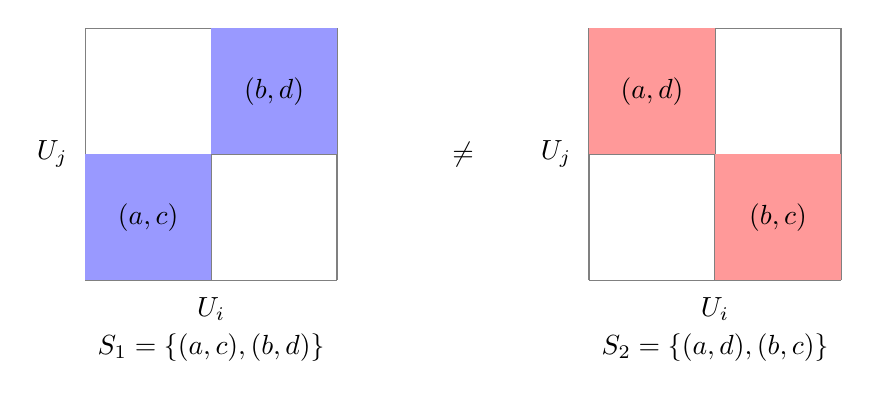
\begin{tikzpicture}[scale=1.6]
    % Left: diagonal {(a,c),(b,d)}
    \draw[step=1cm,gray,thin] (0,0) grid (2,2);
    \fill[blue!40] (0,0) rectangle (1,1);
    \fill[blue!40] (1,1) rectangle (2,2);
    \node at (0.5,0.5) {$(a,c)$}; \node at (1.5,1.5) {$(b,d)$};
    \node[below=0.1cm] at (1,0) {$U_i$};
    \node[left=0.1cm] at (0,1) {$U_j$};
    \node[below=0.55cm] at (1,0) {$S_1=\{(a,c),(b,d)\}$};
    % Right: diagonal {(a,d),(b,c)}
    \draw[step=1cm,gray,thin] (4,0) grid (6,2);
    \fill[red!40] (0,0)++(4,1) rectangle (5,2);
    \fill[red!40] (5,0) rectangle (6,1);
    \node at (4.5,1.5) {$(a,d)$}; \node at (5.5,0.5) {$(b,c)$};
    \node[below=0.1cm] at (5,0) {$U_i$};
    \node[left=0.1cm] at (4,1) {$U_j$};
    \node[below=0.55cm] at (5,0) {$S_2=\{(a,d),(b,c)\}$};
    \node at (3,1) {$\ne$};
  \end{tikzpicture}
  \caption{The constructive witness of
    \url{dichotomy_two_margins}: two non-singleton margins
    $U_i=\{a,b\}$, $U_j=\{c,d\}$ admit two \emph{distinct} full-margin
    subsets $S_1\ne S_2$ of $U_i\times U_j$ --- the two diagonals. Two
    fiber components differing exactly on these diagonals is the
    hole pattern; with at most one non-singleton margin only the full
    rectangle exists ($\mathcal{H}=0$).}
  \label{fig:diagonals}
\end{figure}

\begin{theorem}[T5, Saturation forcing; PROVED]
  \label{thm:t5}
  If a fiber is saturated ($S_r=\mathbb{Z}/D$) and the map
  $A_r$ is a bijection, then $X_r=A_r(S_r)=S_r=Y_r$: no hole; when
  hole-capable, $\sigma=1$.
\end{theorem}

Machine-checked as \url{t5_saturation} (bijective maps send
\url{Finset.univ} to \url{Finset.univ}),
\url{t5_double_saturation} (both fibers saturated), and
\url{t5_sigma_one}. The mechanism behind all six chain-data
suppressions: five instances of type T5(a) at $m=225,441,675,1125$
($S_1=\mathbb{Z}/D$, $D=15/21$) and $m=1800$ (margin-full rectangle,
$A_1$-invariant), and one instance of type T5(b) at $m=675$ with
$r=16$, $r^*=31$ \cite{D199}. No mysterious suppressions remain.

The survey that these theorems explain --- 30 hole-capable pairs, 24
realized, 6 suppressed, all 6 full rectangles ($\delta=0$ both sides;
the strict-subset suppressed case $X=Y\subsetneq R$ never occurs) ---
is [COMPUTED] on two independent paths \cite{D199}; the modulus-level
index $\bar\sigma(m)$ is plotted in
Figure~\ref{fig:sigmabar}.

\begin{figure}[t]
  \centering
  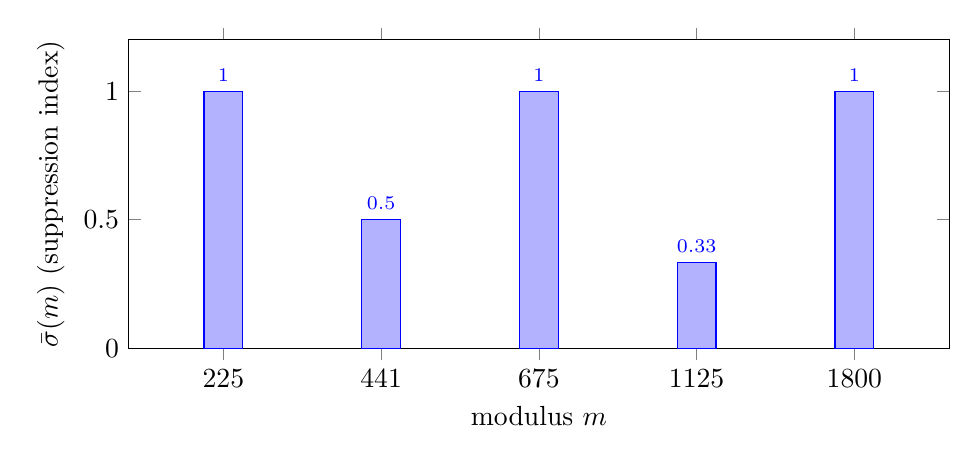
\begin{tikzpicture}
    \begin{axis}[
      ybar, bar width=14pt,
      width=12cm, height=5.5cm,
      ymin=0, ymax=1.2,
      symbolic x coords={225,441,675,1125,1800},
      xtick=data,
      ylabel={$\bar\sigma(m)$ (suppression index)},
      xlabel={modulus $m$},
      nodes near coords, nodes near coords style={font=\scriptsize},
      enlarge x limits=0.15,
    ]
    \addplot coordinates {(225,1.0) (441,0.5) (675,1.0) (1125,0.333) (1800,1.0)};
    \end{axis}
  \end{tikzpicture}
  \caption{Modulus suppression index $\bar\sigma(m)$: fraction of
    hole-capable pairs with $\sigma=1$ (computed datum, R199~\S3).
    Suppression occurs only at these five moduli; all six suppressed
    pairs are full-rectangle T5 instances (Theorem~\ref{thm:t5}).}
  \label{fig:sigmabar}
\end{figure}

\subsection{Absorbed-regime theorems [PROVED]}

\begin{theorem}[T5$'$, no $R\in\{1,2,3,6\}$ non-dead quads; PROVED]
  \label{thm:t5prime}
  Let $m=4c-1$ with $c\ge1$, $m\le2R$, and the per-$R$ automaticity
  conditions ($R=2$: $2\mid c$; $R=3$: $3\mid c$; $R=6$: $2\mid c\land
  3\mid c$). Then $R\in\{1,2,3,6\}$ is impossible, in any regime.
\end{theorem}

Machine-checked as \url{AbsorbedRegime.t5prime_combined}, which
concludes \url{False} from the disjunctive hypothesis, discharging
the four cases via \texttt{t5prime\_R1} ($m\le2$ contradicts $m\ge3$),
\texttt{t5prime\_R2} ($c$ even gives $m\ge7>4$),
\texttt{t5prime\_R3} ($3\mid c$ gives $m\ge11>6$), and
\texttt{t5prime\_R6} ($6\mid c$ gives $m\ge23>12$). The cited premises
(R180's Lemma~2, the $2/3$-automaticity, the $a\le2R/m$ bound chain;
Assumption~\ref{asm:premises}) are the hand-proof inputs; the
machine-checked content is the $m=4c-1$ case analysis. In particular
no absorbed ``un-thinned''/universal-cover quad exists: the
$T=\varnothing$ case is impossible, so a single absorbed quad covers
at most $72<132$ classes \cite{D200}.

\begin{theorem}[T4 corrected, self-bound; PROVED]
  \label{thm:t4corrected}
  An absorbed quad ($13\mid h$, $13\nmid R$) with $R\mid30030$
  satisfies $c\le320$.
\end{theorem}

Machine-checked as \url{AbsorbedBound.t4_self_bound}, with the
bound chain as eight proved lemmas (\S3's
\url{R_dvd_2310} through \url{h_mul_sq_le}). The
machine-checked arithmetic: $13\mid h$ gives $h\ge13$; the
parametrization gives $hm^2\le4R^2$; $R\mid30030$ with $13\nmid R$
gives $R\mid2310$, hence $R\le2310$; so $13m^2\le4\cdot2310^2$,
$m\le1281$, and with $m=4c-1$ this is $c\le320$.

\subsection{The refutation history (reported, not proved)}

The original T4 of the Round~200 dossier read, in full generality:

\begin{proposition}[T4 as stated; REFUTED]
  \label{prop:t4refuted}
  An absorbed quad ($13\mid h$, $13\nmid R$) satisfies $c\le320$.
\end{proposition}

Round~238's hostile review refuted this as stated. The proof began
``$R\mid30030$, $13\nmid R\Rightarrow R\mid2310$,'' but absorption
alone never establishes $R\mid30030$; that hypothesis comes from
non-deadness (R180's Lemma~2, Assumption~\ref{asm:premises}). The
reviewer's counterexample:
\begin{equation}
  \label{eq:counterexample}
  (c,h,a,b)=(321,13,1,16678):\quad a+b=16679=1283\cdot13,
\end{equation}
with $\gcd(ab,h)=1$ and $R=16678\equiv12\pmod{13}$, so $13\nmid R$:
this quad is \emph{absorbed} with $c=321>320$ (dead by Lemma~2, but
absorbed). In fact $(c,13,1,52c-14)$ is absorbed for \emph{every}~$c$
\cite{D238}: the claim ``the $13\mid h$ requirement bounds $c$ by
itself'' is false. Every other step of the proof survived
review (``every remaining step checks out'' \cite{D238}), so the
restored hypothesis in Theorem~\ref{thm:t4corrected} is exactly the
dossier's argument with the missing premise made explicit --- and it
is the restored version that is machine-checked. The uncorrected
Proposition~\ref{prop:t4refuted} is presented here only as a refuted
claim, never as a result.

The same review demoted R200's T2 (trichotomy extension) to
\textbf{[OPEN]}: the unconditional ``$13^1\Vert R$ automatically'' is
false (counterexample $(1,169,169,338)$, for which $R=2\cdot13^2$),
and the fiber formula $s\equiv1-4c\pmod{13}$ lacks its stated premise
\cite{D238}. The conditional core (at a hit, $e-v=1$ and pinning
holds) survived. T3 (fiber-extruded $\kappa$-sub-box) \textbf{survived}
every review step \cite{D238} and stays [PROVED*]; its Lean
formalization needs the $\kappa/\rho/g_0$ apparatus and is not done
here. The 30-quad census (30 absorbed quads with $R\mid30030$, all
dead) stays [COMPUTED] on two parametrizations plus brute force
\cite{D200}.

%======================================================================
\section{Discussion}
%======================================================================

\paragraph{What the formalization buys.} The three modules turn three
previously hand-proved program claims into end-to-end machine-checked
theorems with a pinned toolchain and a closed axiom list. The T2
formalization is not a transcription of the hand proof so much as a
reduction to finite-set combinatorics: the infinite families of fiber
data disappear, leaving ``two distinct full-margin subsets of a
product $\iff$ two non-singleton margins'' --- a statement whose
mechanization is robust to the framework's evolution. The T5$'$ kernel
likewise isolates the $m=4c-1$ arithmetic from the program's
$\kappa$-box machinery, so the impossibility result no longer depends
on any disputed premise.

\paragraph{The review gate works as designed.} Three of the four R200
claims put through hostile review failed as stated --- all on
missing/overbroad hypotheses (unconditional $13^1\Vert R$; the
unstated $R\mid30030$) --- not on the core mathematics, which survived
in every case \cite{D238}. The pattern generalizes: Rounds~233/231 had
the same failure class (the empty set admitted; nine-element
hypotheses omitted) \cite{D238}. The correction of T4 shows the gate's
intended output: a \emph{smaller true theorem} in place of a larger
false one, and the machine-checked version is the corrected one.

\paragraph{Limitations.} (i) The T5$'$ kernel cites the hand-proof
machinery as premises (Assumption~\ref{asm:premises}); only the
$m=4c-1$ arithmetic is machine-checked. (ii) R200's T2 remains [OPEN]
and T3 awaits the $\kappa$-apparatus formalization, so the absorbed
regime's structural theorems are not yet fully mechanized. (iii) The
R199 suppression census and the $m=100$ T3 witness are computational,
not machine-checked; the ``why chain fibers saturate at small
moduli'' question stays [OPEN] \cite{D199}. (iv) The
$\bar\sigma(m)$ plot (Figure~\ref{fig:sigmabar}) is descriptive: no
theorem relates the suppression index to fiber occupancy. (v) The
proofs are constructive elementary arithmetic; no new proof method is
introduced.

%======================================================================
\section{Conclusion}
%======================================================================

We have machine-checked three program results as Lean~4 theorems:
the suppression dichotomy and saturation-forcing of Round~199
(\url{HoleSuppression.t2_iff}, \url{dichotomy_two_margins},
\url{t5_saturation} and variants), the absorbed-regime
$R\in\{1,2,3,6\}$ impossibility of Round~200
(\url{AbsorbedRegime.t5prime_combined} and case lemmas), and the
corrected self-bound \url{AbsorbedBound.t4_self_bound}
(absorbed $+$ $R\mid30030\Rightarrow c\le320$). All are [PROVED]:
exit-0 builds on two machines, zero sorrys, standard-only axioms.
Honestly reported alongside: the refutation of the original T4 (the
$(321,13,1,16678)$ counterexample and the all-$c$ absorbed family),
the demotion of R200's T2 to [OPEN], and the staged statuses of T3,
the 30-quad census, and the R199 surveys. The next mechanization
targets are R200's T3 (fiber-extruded slice, review-cleared) and the
formalization-pending hand-proved backlog.

%======================================================================
\section{References}
%======================================================================

\begin{thebibliography}{9}

\bibitem{D199}
D.~Blair,
\emph{Unsolved Math --- Round 199: hole-suppression theory},
program dossier, 2026-10-09.
(Supplied datum: T1--T5, survey census, $\bar\sigma(m)$ table,
computation details.)

\bibitem{D200}
D.~Blair,
\emph{Unsolved Math --- Round 200: the $13\mid h$ absorbed regime},
program dossier, 2026-10-09.
(Supplied datum: absorbed definition, T2--T5$'$, 30-quad census,
$c\le320$ proof.)

\bibitem{D230}
D.~Blair,
\emph{Unsolved Math --- Round 230: Lean lane --- R222 completion},
program dossier, 2026-10-09.
(Supplied datum: R199 T2/T5 and R200 T5$'$ moved [PROVED];
\url{bakkie} build exit~0, axioms probes.)

\bibitem{D234}
D.~Blair,
\emph{Unsolved Math --- Round 234: Lean lane},
program dossier, 2026-10-09.
(Supplied datum: local elaboration exit~0, 8925 jobs.)

\bibitem{D238}
D.~Blair,
\emph{Unsolved Math --- Round 238: Lean lane},
program dossier, 2026-10-09.
(Supplied datum: hostile review of R200 T2/T3/T4 --- T2 fails as
stated, T3 survives, T4 fails as stated with counterexample
$(321,13,1,16678)$; corrected T4 review-validated;
\url{AbsorbedBound.lean} drafted.)

\bibitem{D250}
D.~Blair,
\emph{Unsolved Math --- Round 250: Lane 4 (Lean formalization)},
program dossier, 2026-10-10.
(Supplied datum: \url{AbsorbedBound.lean} repaired and built
exit~0 on both machines, zero sorrys, standard-only axioms,
md5-identical both sides; corrected T4 \textbf{[PROVED]}.)

\bibitem{Lean}
The Lean~4 theorem prover, v4.34.1; Mathlib v4.34.1 (pinned commit
\url{d13f23b723b8a846827a245b89c10fc7d3f11612}).

\end{thebibliography}

\end{document}

% WEAKNESSES (self-critique, from the author):
% W1. The paper's two halves are formally independent: nothing proved here
%     connects hole suppression (R199) to the absorbed regime (R200). A reader
%     looking for an intellectual through-line gets only the shared review-gate
%     narrative. A joint corollary (e.g. a suppression-style dichotomy inside
%     the absorbed hit set) would have justified one paper instead of two.
% W2. Figure 2 (the sigma-bar plot) is purely descriptive survey data with no
%     theorem attached; it cannot bear weight in any argument. It illustrates
%     context, not mathematics, and the Discussion admits as much.
% W3. The cited premises (Assumption 1: R180 Lemma 2, R184 kappa-set, R196
%     fiber-independence) are load-bearing for T5' and T4 yet entirely outside
%     the machine-checked content; the paper inherits their truth value from
%     the dossiers. The staged-verification caveats partly mitigate this, but
%     a hostile reader can fairly ask what exactly was machine-checked.
% TYPOGRAPHY ISSUES NOTICED:
% T1. Table 1's status column mixes \textbf{} (REFUTED, [OPEN]) with plain
%     [PROVED]; the emphasis is justified by honesty but the column is ragged
%     in width -- consider a fixed-width p-column or centering.
% T2. The theorem names in teletype (t2_iff etc.) wrap awkwardly in the
%     booktabs table; \texttt breaks poorly at column boundaries -- consider
%     \seqsplit or short names with a lookup appendix.
% T3. Figure 1's grid labels: the (a,d)/(b,c) cell coordinates in the right
%     sub-grid are placed by absolute shift (4,1)/(5,0); if the TikZ scale or
%     grid origin changes, the fill rectangles and node labels can desync --
%     prefer relative positioning from the grid corners.
